\chapter{p3 = 38 (5 graphs)}
\newpage\begin{figure}
  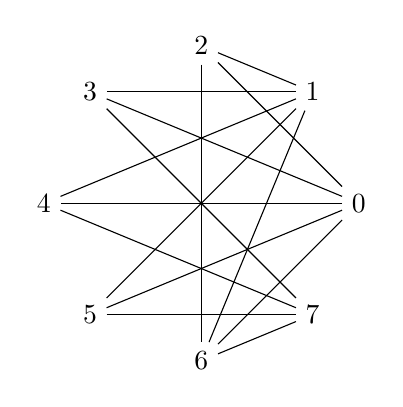
\begin{tikzpicture}
      \draw
        (0.0:2) node (0){0}
        (45.0:2) node (1){1}
        (90.0:2) node (2){2}
        (135.0:2) node (3){3}
        (180.0:2) node (4){4}
        (225.0:2) node (5){5}
        (270.0:2) node (6){6}
        (315.0:2) node (7){7};
      \begin{scope}[-]
        \draw (0) to (2);
        \draw (0) to (3);
        \draw (0) to (4);
        \draw (0) to (5);
        \draw (0) to (6);
        \draw (1) to (2);
        \draw (1) to (3);
        \draw (1) to (4);
        \draw (1) to (5);
        \draw (1) to (6);
        \draw (2) to (6);
        \draw (3) to (7);
        \draw (4) to (7);
        \draw (5) to (7);
        \draw (6) to (7);
      \end{scope}
    \end{tikzpicture}
\end{figure}
\begin{itemize}
\item signature: 0111110111110000100001001011
\item g: Graph with 8 nodes and 15 edges
\item order: 8
\item size: 15
\item max degree: 5
\item degrees: 3,3,3,3,4,4,5,5
\item is tree: 0
\item is bipartite: 0
\item has bridge: 0
\item is chordal: 0
\item is complete: 0
\item min cycle basis weight: 30
\item min cycle basis size: 8
\item diameter: 2
\item radius: 2
\item is eulerian: 0
\item is planar: 0
\item number of faces: 9
\item is regular: 0
\item p3: 38
\item p4: None
\item property hash: 5ed1f20cd375cd88432e204968e60a542571e188cba50a2f3fb9082549b42922
\end{itemize}
\newpage
\begin{figure}
  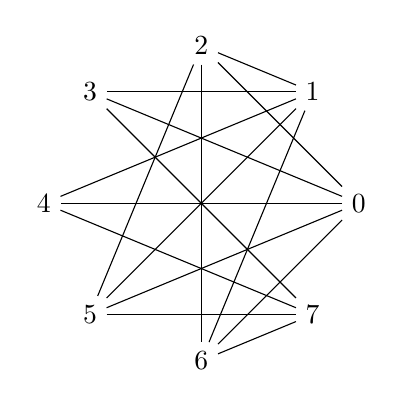
\begin{tikzpicture}
      \draw
        (0.0:2) node (0){0}
        (45.0:2) node (1){1}
        (90.0:2) node (2){2}
        (135.0:2) node (3){3}
        (180.0:2) node (4){4}
        (225.0:2) node (5){5}
        (270.0:2) node (6){6}
        (315.0:2) node (7){7};
      \begin{scope}[-]
        \draw (0) to (2);
        \draw (0) to (3);
        \draw (0) to (4);
        \draw (0) to (5);
        \draw (0) to (6);
        \draw (1) to (2);
        \draw (1) to (3);
        \draw (1) to (4);
        \draw (1) to (5);
        \draw (1) to (6);
        \draw (2) to (5);
        \draw (2) to (6);
        \draw (3) to (7);
        \draw (4) to (7);
        \draw (5) to (7);
        \draw (6) to (7);
      \end{scope}
    \end{tikzpicture}
\end{figure}
\begin{itemize}
\item signature: 0111110111110001100001001011
\item g: Graph with 8 nodes and 16 edges
\item order: 8
\item size: 16
\item max degree: 5
\item degrees: 3,3,4,4,4,4,5,5
\item is tree: 0
\item is bipartite: 0
\item has bridge: 0
\item is chordal: 0
\item is complete: 0
\item min cycle basis weight: 32
\item min cycle basis size: 9
\item diameter: 2
\item radius: 2
\item is eulerian: 0
\item is planar: 0
\item number of faces: 10
\item is regular: 0
\item p3: 38
\item p4: None
\item property hash: 0b51ed17cc6f3d1896ebf27b3b9504a468ec80781091f7f77fe28e19f6aeb0d3
\end{itemize}
\newpage
\begin{figure}
  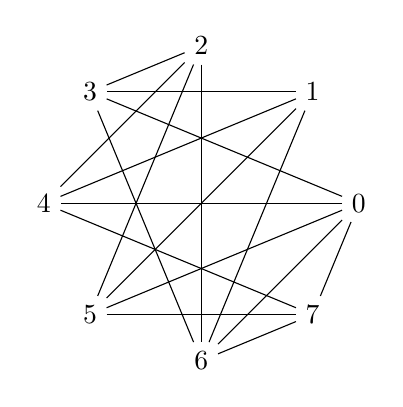
\begin{tikzpicture}
      \draw
        (0.0:2) node (0){0}
        (45.0:2) node (1){1}
        (90.0:2) node (2){2}
        (135.0:2) node (3){3}
        (180.0:2) node (4){4}
        (225.0:2) node (5){5}
        (270.0:2) node (6){6}
        (315.0:2) node (7){7};
      \begin{scope}[-]
        \draw (0) to (3);
        \draw (0) to (4);
        \draw (0) to (5);
        \draw (0) to (6);
        \draw (0) to (7);
        \draw (1) to (3);
        \draw (1) to (4);
        \draw (1) to (5);
        \draw (1) to (6);
        \draw (2) to (3);
        \draw (2) to (4);
        \draw (2) to (5);
        \draw (2) to (6);
        \draw (3) to (6);
        \draw (4) to (7);
        \draw (5) to (7);
        \draw (6) to (7);
      \end{scope}
    \end{tikzpicture}
\end{figure}
\begin{itemize}
\item signature: 0011111011110111100010001011
\item g: Graph with 8 nodes and 17 edges
\item order: 8
\item size: 17
\item max degree: 5
\item degrees: 4,4,4,4,4,4,5,5
\item is tree: 0
\item is bipartite: 0
\item has bridge: 0
\item is chordal: 0
\item is complete: 0
\item min cycle basis weight: 34
\item min cycle basis size: 10
\item diameter: 2
\item radius: 2
\item is eulerian: 0
\item is planar: 0
\item number of faces: 11
\item is regular: 0
\item p3: 38
\item p4: None
\item property hash: 87c17f84b1d00d3ef9c9e5c1e501ca29af6bfb59b33684dce6f6936f719b97e8
\end{itemize}
\newpage
\begin{figure}
  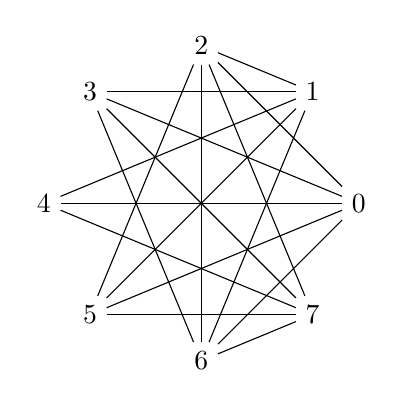
\begin{tikzpicture}
      \draw
        (0.0:2) node (0){0}
        (45.0:2) node (1){1}
        (90.0:2) node (2){2}
        (135.0:2) node (3){3}
        (180.0:2) node (4){4}
        (225.0:2) node (5){5}
        (270.0:2) node (6){6}
        (315.0:2) node (7){7};
      \begin{scope}[-]
        \draw (0) to (2);
        \draw (0) to (3);
        \draw (0) to (4);
        \draw (0) to (5);
        \draw (0) to (6);
        \draw (1) to (2);
        \draw (1) to (3);
        \draw (1) to (4);
        \draw (1) to (5);
        \draw (1) to (6);
        \draw (2) to (5);
        \draw (2) to (6);
        \draw (2) to (7);
        \draw (3) to (6);
        \draw (3) to (7);
        \draw (4) to (7);
        \draw (5) to (7);
        \draw (6) to (7);
      \end{scope}
    \end{tikzpicture}
\end{figure}
\begin{itemize}
\item signature: 0111110111110001110011001011
\item g: Graph with 8 nodes and 18 edges
\item order: 8
\item size: 18
\item max degree: 5
\item degrees: 3,4,4,5,5,5,5,5
\item is tree: 0
\item is bipartite: 0
\item has bridge: 0
\item is chordal: 0
\item is complete: 0
\item min cycle basis weight: 35
\item min cycle basis size: 11
\item diameter: 2
\item radius: 2
\item is eulerian: 0
\item is planar: 0
\item number of faces: 12
\item is regular: 0
\item p3: 38
\item p4: None
\item property hash: aea2e239b24f3f60a822c5e3986aee0c9162de2ad0db49ef7baa0da55522ef7d
\end{itemize}
\newpage
\begin{figure}
  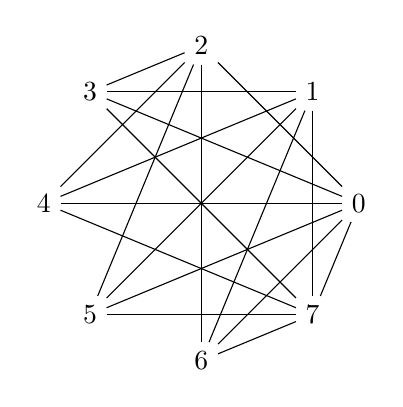
\begin{tikzpicture}
      \draw
        (0.0:2) node (0){0}
        (45.0:2) node (1){1}
        (90.0:2) node (2){2}
        (135.0:2) node (3){3}
        (180.0:2) node (4){4}
        (225.0:2) node (5){5}
        (270.0:2) node (6){6}
        (315.0:2) node (7){7};
      \begin{scope}[-]
        \draw (0) to (2);
        \draw (0) to (3);
        \draw (0) to (4);
        \draw (0) to (5);
        \draw (0) to (6);
        \draw (0) to (7);
        \draw (1) to (3);
        \draw (1) to (4);
        \draw (1) to (5);
        \draw (1) to (6);
        \draw (1) to (7);
        \draw (2) to (3);
        \draw (2) to (4);
        \draw (2) to (5);
        \draw (2) to (6);
        \draw (3) to (7);
        \draw (4) to (7);
        \draw (5) to (7);
        \draw (6) to (7);
      \end{scope}
    \end{tikzpicture}
\end{figure}
\begin{itemize}
\item signature: 0111111011111111100001001011
\item g: Graph with 8 nodes and 19 edges
\item order: 8
\item size: 19
\item max degree: 6
\item degrees: 4,4,4,4,5,5,6,6
\item is tree: 0
\item is bipartite: 0
\item has bridge: 0
\item is chordal: 0
\item is complete: 0
\item min cycle basis weight: 36
\item min cycle basis size: 12
\item diameter: 2
\item radius: 2
\item is eulerian: 0
\item is planar: 0
\item number of faces: 13
\item is regular: 0
\item p3: 38
\item p4: None
\item property hash: b316b0540b66d2431ca1cb0ad25cb7ef8a899d93d8accb2afe000a5f0ea295ad
\end{itemize}
\newpage
